\documentclass[11pt]{ecsarticle}
\usepackage[nodayofweek]{datetime}
\usepackage{natbib} 
\usepackage{graphicx}
\usepackage{caption}
\usepackage{subcaption}



\title{COMP6026 - Assignment 2 - Group Selection}
\authors{Henry Lovett - hl13g10}
\begin{document}
\maketitle
 
\section{Introduction}

This work is based on \cite{powers2007individual}.

Describe paper/experiment.
Game theory game - defectors win CITE


How individuals were represented

Group allocation

Resource equation \& explanation

Growth equation \& explanation



\section{Reimplementation}
\begin{figure}
        \centering
        \begin{subfigure}[b]{0.4\textwidth}
                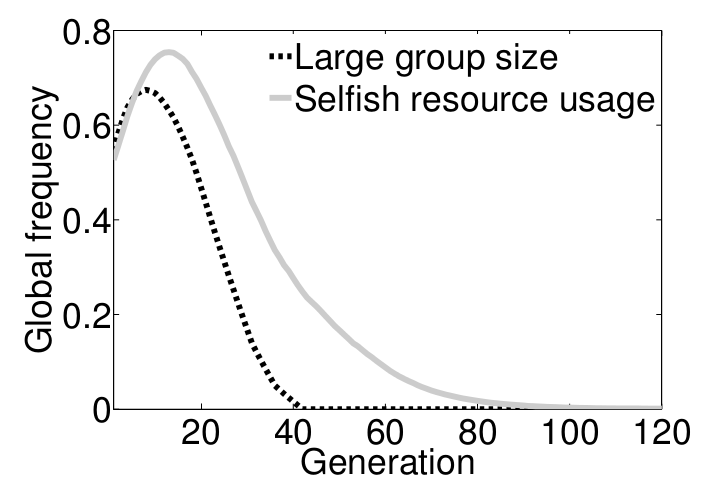
\includegraphics[width=\textwidth]{orig_a.png}
                \caption{Average Environment and strategy through time.}
                \label{fig:orig:A}
        \end{subfigure}%
        ~ %add desired spacing between images, e. g. ~, \quad, \qquad etc.
          %(or a blank line to force the subfigure onto a new line)
        \begin{subfigure}[b]{0.4\textwidth}
                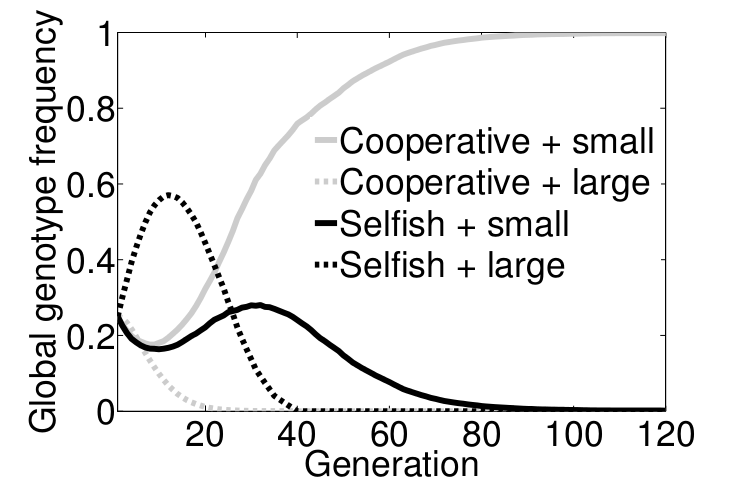
\includegraphics[width=\textwidth]{orig_b.png}
                \caption{Change in genotype frequencies over time.}
                \label{fig:orig:B}
        \end{subfigure}
        \caption{The original results from \cite{powers2007individual}.}\label{fig:animals}
\end{figure}

\begin{figure}
        \centering
        \begin{subfigure}[b]{0.4\textwidth}
                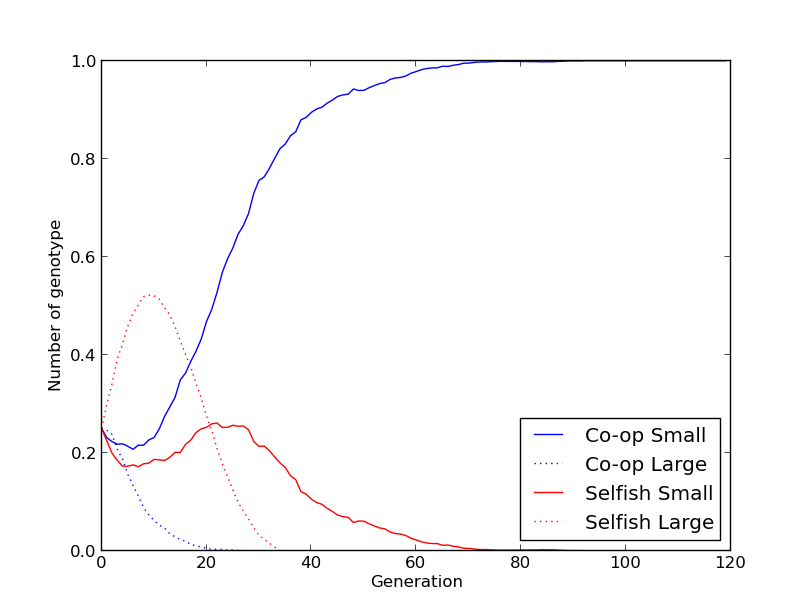
\includegraphics[width=\textwidth]{Code2/fig1.png}
                \caption{Average Environment and strategy through time.}
                \label{fig:rep:A}
        \end{subfigure}%
        ~ %add desired spacing between images, e. g. ~, \quad, \qquad etc.
          %(or a blank line to force the subfigure onto a new line)
        \begin{subfigure}[b]{0.4\textwidth}
                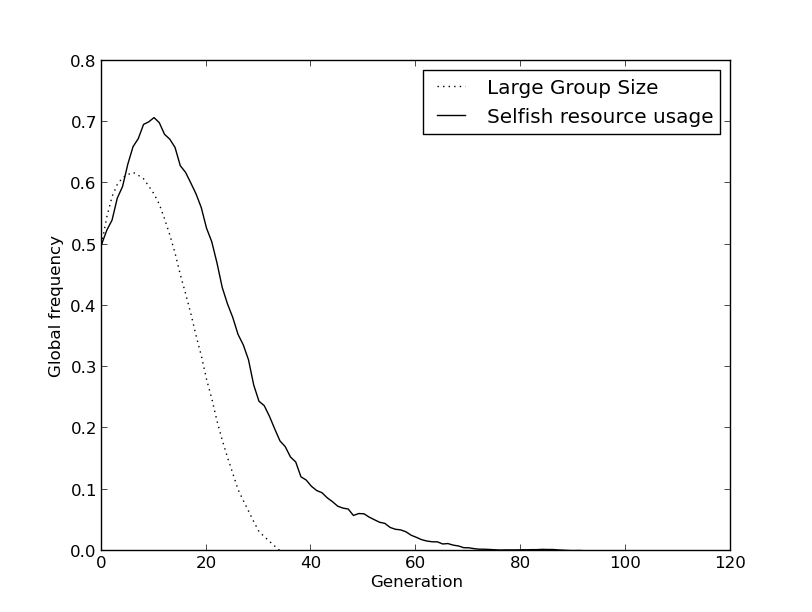
\includegraphics[width=\textwidth]{Code2/fig2.png}
                \caption{Change in genotype frequencies over time.}
                \label{fig:rep:B}
        \end{subfigure}
        \caption{Reproduced results.}\label{fig:animals}
\end{figure}
\section{Extension}

\section{Results}

\section{Conclusion}


\bibliographystyle{apalike}
\bibliography{bibliography}
 
\end{document}
